\documentclass[11pt, letterpaper]{article}
\usepackage[in]{fullpage}
\usepackage{enumerate}
\usepackage{amsmath}
\usepackage{graphicx}
\title{CS301 Project 1\\Image Warping and Mosaic} 
\author{ Matt  Nuckolls \\ 
         Michael Wisely \\ } 
\date{\today}
\begin{document}
\maketitle

\section{Project Goals}
In this project, a MATLAB program was designed to stitch two images
together to create a larger mosaic. The program first showed the user
a source image, allowing him to click four image features that laid on
a planar surface in the image. After pressing ``enter'', the user was
shown the destination image and chose the same four feature
points. After pressing ``enter'' a second time, the program calculated
a homogrphy matrix that mapped points from the source image into the
destination image. The program then used a warping technique to
transform the source image so that it had the four selected points
from both images would be in the same plane. The images were then
``stitched'' together using an image stitching algorithm, and the
result was shown to the user.

The aim of this project was to gain a better understanding of
homography matrices, image warping, and MATLAB programming by
implementing image warping and stitching algorithms in MATLAB. This
project also allowed developers to compare the different algorithms
that were used to compute homography matrices, warp images, and stitch
images together.

\begin{figure}[here]
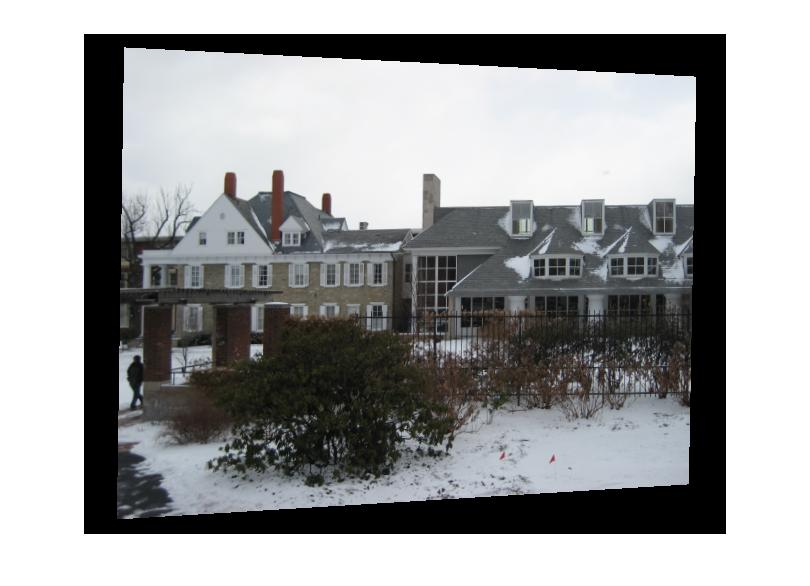
\includegraphics[width=\textwidth]{../pics/snow-backward-bilinear-warp.jpg}
\caption{Image Warping}
\end{figure}

\section{Homographies}
The purpose of a homography in this context is to map points from one
projected plane in an image to points in a projected plane from a
different image. This is particularly useful when stitching images
together. Images that are taken at different perspectives can be
transformed using a homography so that they all lie in the same
plane. The images can then be placed next to one another or overlapped
to create a single image with a broader view. 

In this project, homography matrices were calculated using two methods:
the pseudo-inverse method and the single value decomposition method.

\paragraph{The Pseudo-Inverse Method}
Using the pseudo-inverse method, we first assume that $h_{33}$ of the
homography matrix will be 1. 

\[
\begin{bmatrix}
  x' \\  y' \\  1
\end{bmatrix}
\sim 
\begin{bmatrix}
  h_{11} & h_{12} & h_{13} \\
  h_{21} & h_{22} & h_{23} \\
  h_{31} & h_{32} & 1 
\end{bmatrix}
\begin{bmatrix}
  x \\  y \\  1
\end{bmatrix}
\]

We can then perform matrix multiplication to develop a system of
linear equations relating $x'$ and $y'$ to $x$, $y$, and the elements
of the homography matrix. These equations can be rearranged so that
unknown variables are the elements of the homography matrix.

\[
\begin{bmatrix}
  x_1 & y_1 & 1 & 0 & 0 & 0 & -x_1x'_1 & -y_1x'_1 \\
  0 & 0 & 0 & x_1 & y_1 & 1 & -x_1y'_1 & -y_1y'_1 \\
  x_2 & y_2 & 2 & 0 & 0 & 0 & -x_2x'_2 & -y_2x'_2 \\
  0 & 0 & 0 & x_2 & y_2 & 2 & -x_2y'_2 & -y_2y'_2 \\
  x_3 & y_3 & 3 & 0 & 0 & 0 & -x_3x'_3 & -y_3x'_3 \\
  0 & 0 & 0 & x_3 & y_3 & 3 & -x_3y'_3 & -y_3y'_3 \\
  x_4 & y_4 & 4 & 0 & 0 & 0 & -x_4x'_4 & -y_4x'_4 \\
  0 & 0 & 0 & x_4 & y_4 & 4 & -x_4y'_4 & -y_4y'_4 
\end{bmatrix}
\begin{bmatrix}
  h_{11} \\ h_{12} \\ h_{13} \\ h_{21} \\ h_{22} \\ h_{23} \\ h_{31} \\ h_{32} 
\end{bmatrix}
=
\begin{bmatrix}
  x'_1 \\ y'_1 \\ x'_2 \\ y'_2 \\ x'_3 \\ y'_3 \\ x'_4 \\ y'_4
\end{bmatrix}
\]

Or more compactly...
\[
\mathbf{A}\mathbf{h}=\mathbf{b}
\]

By creating a new matrix for these equations, we can solve for the
homography matrix a couple of ways. We can either compute a
pseudo-inverse by doing
$\mathbf{h}=(\mathbf{A}^T\mathbf{A})^{-1}(\mathbf{A}^T\mathbf{b})$ or
we can use $\mathbf{h}=\mathbf{A}\backslash\mathbf{b}$ in MATLAB.

We chose to use $\mathbf{h}=\mathbf{A}\backslash\mathbf{b}$ to compute
the homography with our pseudo inverse method. This operator was
obviously faster than
$\mathbf{h}=(\mathbf{A}^T\mathbf{A})^{-1}(\mathbf{A}^T\mathbf{b})$,
taking 0.000149 seconds instead of 0.062804 seconds according to
\emph{tic} and \emph{toc}. Because the longer operation also used
matrix inverse, MATLAB warned that the result may be
inaccurate. However, any errors that may have been present were not
visible in the image to the naked eye.

\paragraph{The Single Value Decomposition Method}
Instead of constraining $h_{33}$ to 1, the SVD method constrains the
norm of h, $\|h\|$ to 1. This allows the value of $h_{33}$ to be 0,
which is obviously not possible with the pseudo-inverse method. To
compute a homography matrix using SVD, we must create a set of linear
equations, much like we did for psuedo-inverse, with the elements of
the homography matrix as unknowns. This time, however, we arrange the
euqations slightly differently.

\[
\begin{bmatrix}
  x_1 & y_1 & 1 & 0 & 0 & 0 & -x_1x'_1 & -y_1x'_1 -x'_1 \\
  0 & 0 & 0 & x_1 & y_1 & 1 & -x_1y'_1 & -y_1y'_1 -y'_1 \\
  x_2 & y_2 & 2 & 0 & 0 & 0 & -x_2x'_2 & -y_2x'_2 -x'_2 \\
  0 & 0 & 0 & x_2 & y_2 & 2 & -x_2y'_2 & -y_2y'_2 -y'_2 \\
  x_3 & y_3 & 3 & 0 & 0 & 0 & -x_3x'_3 & -y_3x'_3 -x'_3 \\
  0 & 0 & 0 & x_3 & y_3 & 3 & -x_3y'_3 & -y_3y'_3 -y'_3 \\
  x_4 & y_4 & 4 & 0 & 0 & 0 & -x_4x'_4 & -y_4x'_4 -x'_4 \\
  0 & 0 & 0 & x_4 & y_4 & 4 & -x_4y'_4 & -y_4y'_4 -y'_4
\end{bmatrix}
\begin{bmatrix}
  h_{11} \\ h_{12} \\ h_{13} \\ h_{21} \\ h_{22} \\ h_{23} \\ h_{31} \\ h_{32} 
\end{bmatrix}
=
\begin{bmatrix}
  0 \\   0 \\   0 \\   0 \\   0 \\   0 \\   0 \\   0 \\   0 
\end{bmatrix}
\]

Or, again, more compactly...
\[
\mathbf{A}\mathbf{h}=\mathbf{0}
\]

To solve this matrix equation, we cannot perform a matrix inverse as
we did before because $\mathbf{A}\mathbf{0}$ will allways be
$\mathbf{0}$. Instead, can either perform computations involving
eigenvalues, or we use MATLAB's SVD function. For simplicity and
speed, we chose to use the SVD function. This function returns several
items, but our item of interest was the last column of $\mathbf{V}^T$,
which corresponded to the values in our homography matrix.

Neither method was particularly more difficult to implement than the
other, especially considering the convenience functions offered by
MATLAB. The homography matrix generated by each method was the same,
but off by a scalar multiple. 

Below is a snipped of a MATLAB session that shows the similarities
between the homography generated by the pseudo-inverse method and the
SVD method. The ``h1'' variable holds the pseudo-inverse homography,
its $h_{33}=1$, and the ``h2'' variable holds the SVD homography. By
scaling h2 by its $h_{33}$ value, we can see that the matrices are the
same (as they should be).

\begin{verbatim}
h1 =

    1.1804   -0.0167 -196.4375
    0.0636    1.1141  -20.5098
    0.0003    0.0000    1.0000


h2 =

    0.0060   -0.0001   -0.9945
    0.0003    0.0056   -0.1038
    0.0000    0.0000    0.0051

>> h2 * 1/h2(3,3)
ans =

    1.1804   -0.0167 -196.4375
    0.0636    1.1141  -20.5098
    0.0003    0.0000    1.0000
\end{verbatim}

\section{Warping}
After computing the homography matrix, one must apply the homography
to each pixel in an image to warp it to a new projected plane. This
can be accomplished several different ways. For this project, three
different methods were used: forward warping, backward warping, and
interp2.

\paragraph{Forward Warping}
To forward warp, we first create an solid black, empty image which
will hold the result of the warp. We then use nested for loops to
iterate through each pixel in the source image, applying the
homography matrix to each one. The result gives us the coordinates for
each pixel in the resulting image. We can then copy the color value
for each pixel to the appropriate locations in the resulting
image. 

The disadvantage to this is that the method maps every pixel in the
source to a location in the result, but not every result is covered by
a source pixel. Each spot in the result that was not covered by a
pixel in the source is left black. This leaves us with a grid of black
lines on the resulting warped image (see Figure
~\ref{fig:forwardWarping}). These lines can be corrected by processing
the image after warping it.

\begin{figure}[here]
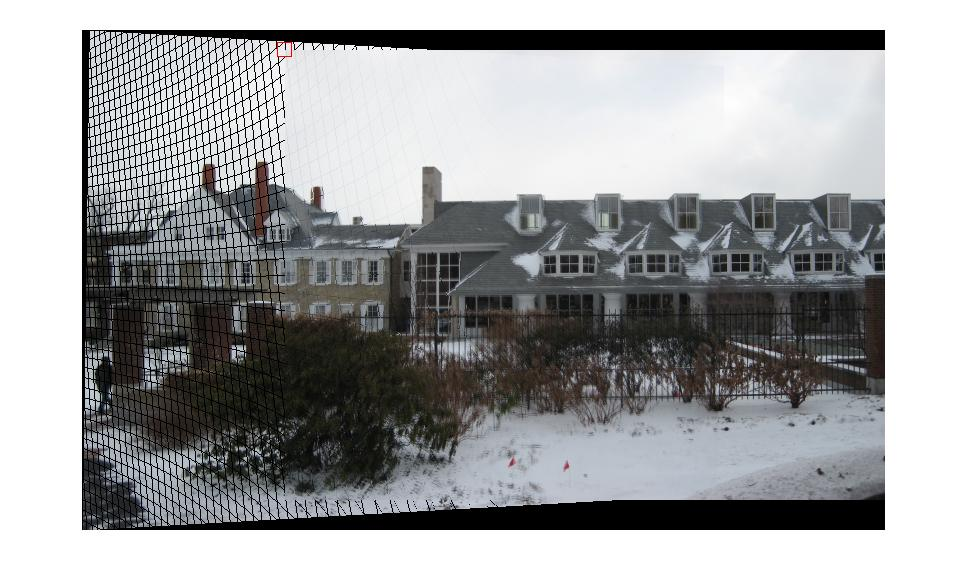
\includegraphics[width=\textwidth]{../pics/snow-svd-forward-blended.jpg}
\caption{Forward Warping with SVD Homography and Blended Mosaic}
\label{fig:forwardWarping}
\end{figure}

\paragraph{Backward Warping}
To backward warp, we first create an solid black, empty image which
will hold the result of the warp. We then use nested for loops to
iterate through each pixel in the \emph{empty} image, and instead,
apply $\mathbf{h}^{-1}$ to each pixel, to determine which pixel in the
source should map to that location. If the calculated location is
outside of the bounds of the source image, we ignore it. If the
location is within the image, it is unlikely that we will land
directly on a pixel. Instead, we will likely land at a location that
is between pixels. 

To determine the color value for a pixel in the warped image, we have
several options. The easiest option is to round the x and
y coordinates of the result, and use that color value found at that pixel. This is called
the \emph{nearest} interpolation method (see Figure
~\ref{fig:backwardNearestWarping}). The other option is to take a
weigted average of the pixels surrounding the calculated
location. This method is called the \emph{bilinear} interpolation
method (see Figure ~\ref{fig:backwardBilinearWarping}). By closely
inspecting the two produced images, one can see that the nearest
interpolation method produces a blockier image than the bilinear
method. The bilinear backward warped image looks smoother.


\begin{figure}[here]
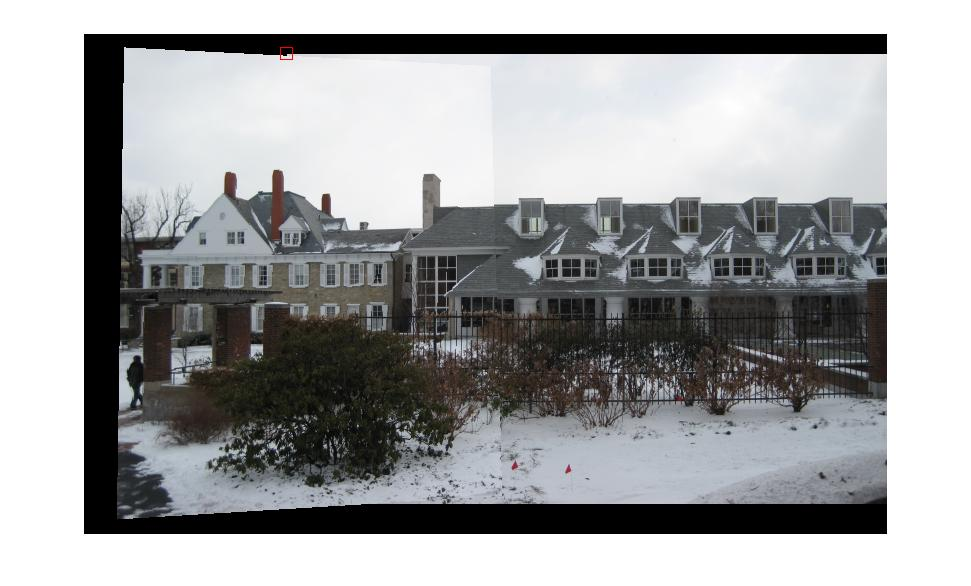
\includegraphics[width=\textwidth]{../pics/snow-svd-backward-nearest-nearest.jpg}
\caption{Backward Warping with Nearest Interpolation, 
  SVD Homography, and Nearest Mosaic}
\label{fig:backwardNearestWarping}
\end{figure}

\begin{figure}[here]
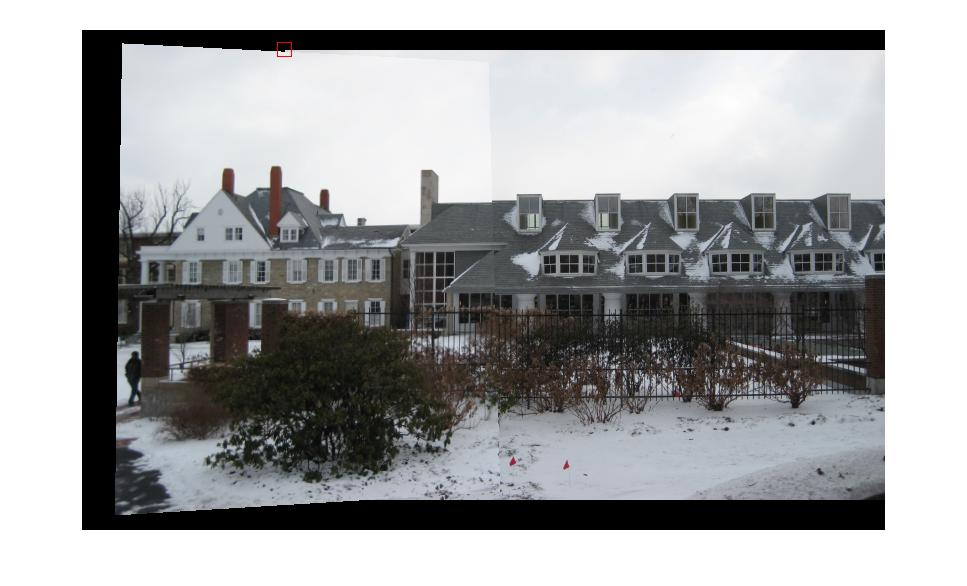
\includegraphics[width=\textwidth]{../pics/snow-svd-backward-bilinear-nearest.jpg}
\caption{Backward Warping with Bilinear Interpolation, 
  SVD Homography, and Nearest Mosaic}
\label{fig:backwardBilinearWarping}
\end{figure}


\paragraph{Interp2}
MATLAB provides a function named interp2, which can perform warping
and interpolation. The results of this warp look very smooth, and
appear to match the destination image the best. However, in our
experience, it cropped the side of our image, and the mosaic looks
strange (see Figure ~\ref{fig:interp2Warping}).

\begin{figure}[here]
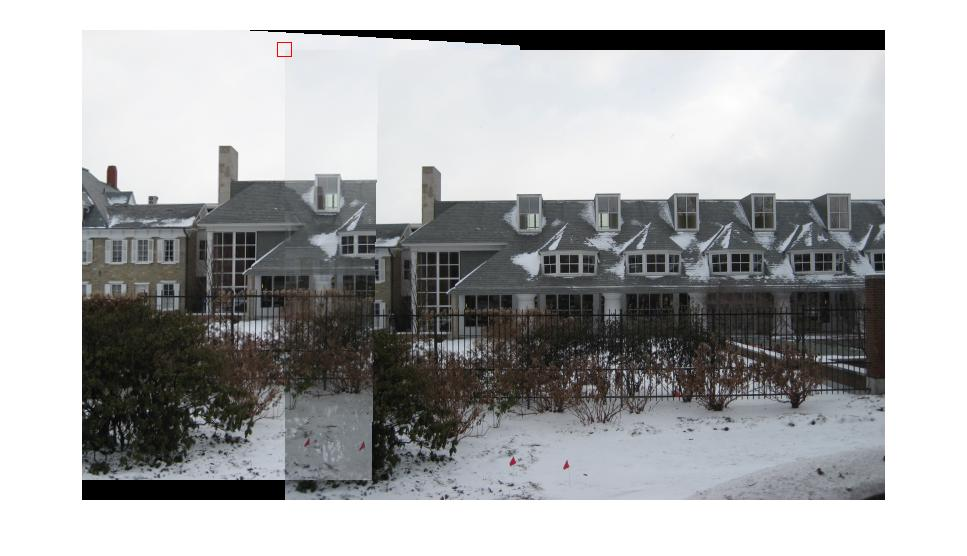
\includegraphics[width=\textwidth]{../pics/snow-svd-interp2-blended.jpg}
\caption{Interp2 Warping, SVD Homography, and Blended Mosaic}
\label{fig:interp2Warping}
\end{figure}

\paragraph{Summary}
Of the three interpolation options, interp2 was obviously the
fastest. It is a MATLAB function, and makes use of high performance
code behind the scenes. The for-loop method used with backward and
forward warping tooks seconds, if not minutes, to complete, while the
interp2 function took a fraction of a second. However, because interp2
cropped part of our image, the resulting mosaic image appeared
strange. The backward warping method with bilinear interpolation
produced the best warped mosaic.

\section{Mosaic}
After warping a source image to match the same projected plane as the
destination image, one must put the two images together. We used two
different methods to accomplish this. The ``nearest'' method (Figure
~\ref{fig:backwardBiliniearWarping}) considers the area where the two
images overlap, and for each pixel, determines whether the source
pixel or the destination pixel should be chosen based on whether it is
closer to the source's center of mass or the destination's center of
mass. Similarly, the ``blended'' method (Figure
~\ref{fig:forwardWarping}) considers overlapping areas, but takes a
weighted average of the source and destination pixels at that spot and
adds that result to the mosaic.

\section{Design Decisions}
The general flow of the program can be seen in Figure ~\ref{fig:flowChart}.

\begin{figure}[here]
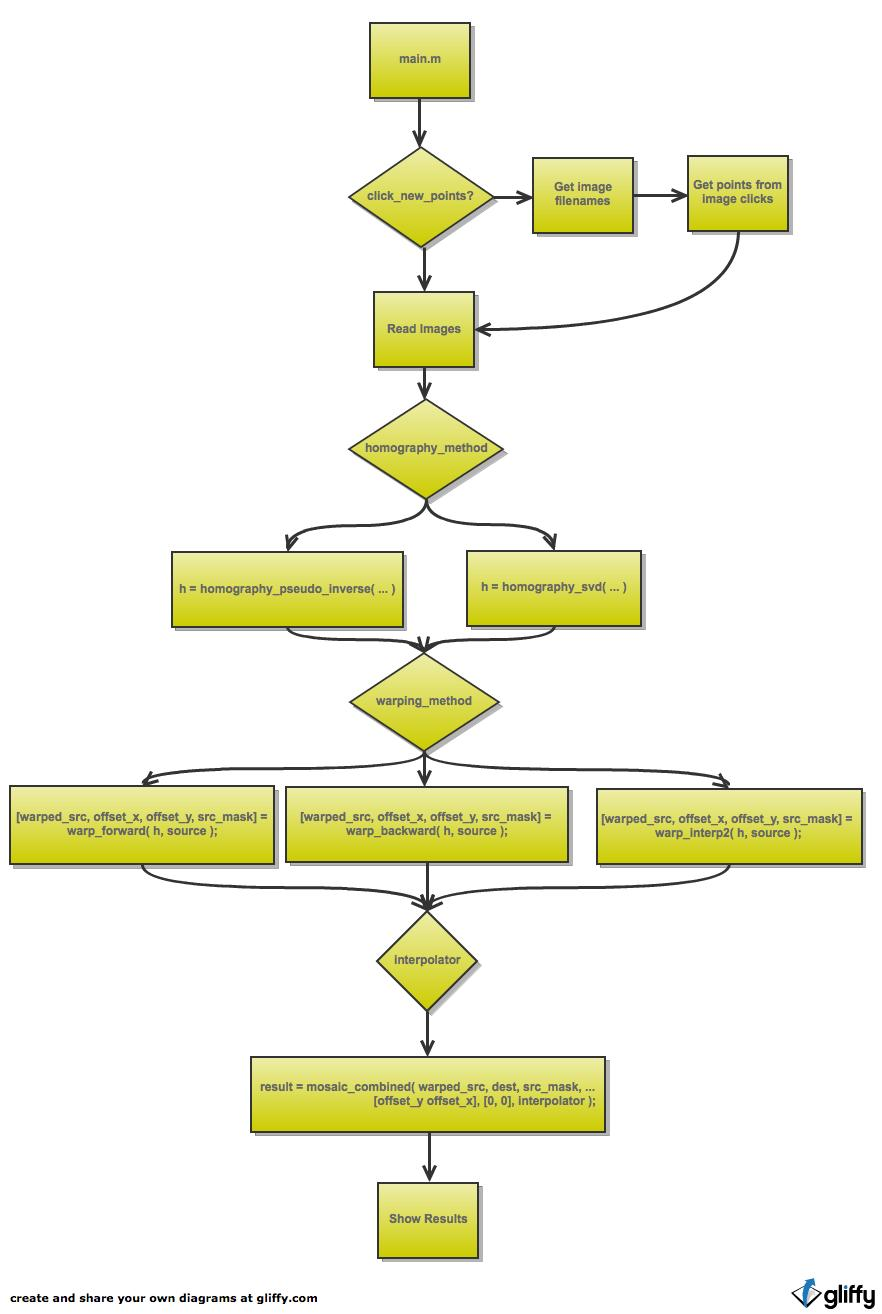
\includegraphics[width=.8\textwidth]{./flowchart.jpg}
\caption{High Level Flow Control}
\label{fig:flowChart}
\end{figure}

\paragraph{User Configuration}
To make this program flexible for the user, several configuration
options are provided at the beginning of main.m.

\begin{description}
\item[click\_new\_points] \hfill \\
  Can be {\bf yes} or {\bf no}. If yes, the program will prompt the user
  for image files to warp together, and it will ask them to manually
  select points in those images. If no, the program will use the default
  ``snow'' images and use preselected points. The no option is for
  debugging.
  
\item[homography\_method] \hfill \\
  Can be {\bf pseudo\_inverse} or {\bf svd}. Determines which method
  should be used to calculate the homography matrix.
  
\item[warping\_method] \hfill \\
  Can be {\bf forward}, {\bf backward}, or {\bf interp2}. This option
  allows the user to decide which warping method to use. The default
  interpolation for backward warping is ``bilinear'', but it can be
  changed to the blocker ``nearest'' by uncommenting a line in
  warp\_backward.m.
\end{description}

%% TODO Add something about masks

\section{Experimental Observations}
%% TODO Make sure this is correct 
Overall, things turned out the way we expected. This project was fun
and interesting to work on, though neither of us are huge fans of
MATLAB. We decided that MATLAB is a great tool for image processing
because of its vector and matrix features, allowing for complex
slicing and manipulation of those data structures. These features
allowed for easier and faster manipulation of images.

%% TODO Gah. I am running out of brain

\section{Group Contribution}
\paragraph{Matt}
Matt developed the homography computation code, the warping code, and
the main MATLAB script. He also contributed to the report.

\paragraph{Michael}
Michael worked on the mosaic code and contributed to the warping
code. He worked on much of the report.

\end{document}
